\begin{figure}[H]
\centering
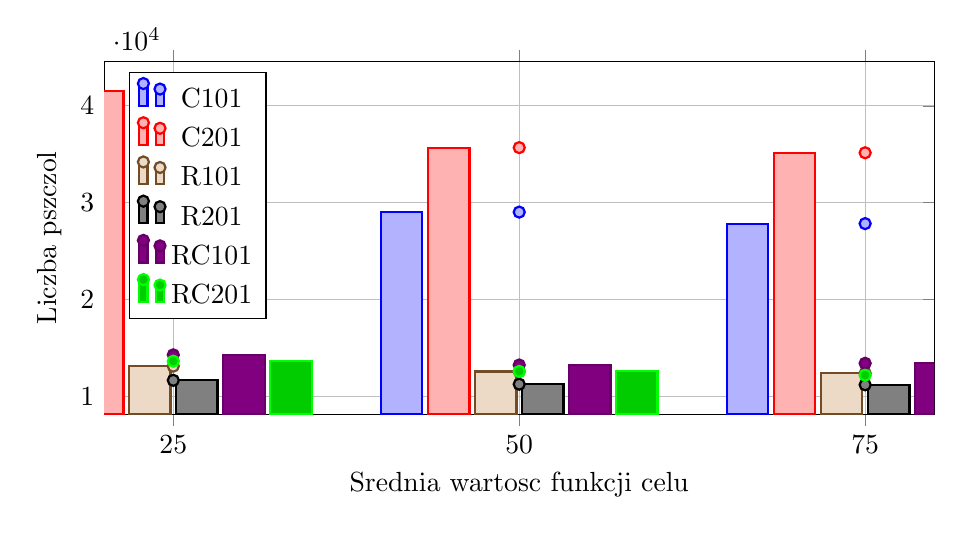
\begin{tikzpicture}
\begin{axis}[
xlabel = {Srednia wartosc funkcji celu},
ylabel = {Liczba pszczol},
legend pos = north west,
grid = both,
width=1\linewidth,
height=0.5\linewidth,
ybar,
bar width=15pt,
symbolic x coords={25,50,75,},
xtick=data
]
\addplot + [mark = *, thick] coordinates
    {
(25,30199.875)(50,29015.5)(75,27825.25)};
\addlegendentry
{C101}
\addplot + [mark = *, thick] coordinates
    {
(25,41554.0)(50,35676.625)(75,35144.5)};
\addlegendentry
{C201}
\addplot + [mark = *, thick] coordinates
    {
(25,13094.25)(50,12537.875)(75,12372.625)};
\addlegendentry
{R101}
\addplot + [mark = *, thick] coordinates
    {
(25,11635.75)(50,11236.625)(75,11172.625)};
\addlegendentry
{R201}
\addplot + [mark = *, thick] coordinates
    {
(25,14266.875)(50,13217.875)(75,13394.0)};
\addlegendentry
{RC101}
\addplot + [mark = *, thick] coordinates
    {
(25,13612.875)(50,12558.75)(75,12159.375)};
\addlegendentry
{RC201}
\end{axis}
\end{tikzpicture}
\caption
{Srednia wartosc funkcji celu w zaleznosci od liczby pszczol dla poszczegolnych instancji}
\label{fig:mean_goals_per_bee_number_per_instance}
\end{figure}
